\documentclass[10pt,a4paper]{article}
\usepackage[utf8]{inputenc}
\usepackage[german]{babel}
\usepackage[T1]{fontenc}
\usepackage{amsmath}
\usepackage{amsfonts}
\usepackage{amssymb}
\usepackage{tabularx}
\usepackage{ltablex}
\usepackage{graphicx}
\graphicspath{{images/}}
\usepackage{subcaption}
\usepackage{cite}
\usepackage[nottoc,numbib]{tocbibind}
\usepackage{hyperref}
\hypersetup{
    colorlinks,
    citecolor=black,
    filecolor=black,
    linkcolor=black,
    urlcolor=black
}
\usepackage{sectsty}

\author{Christopher Besch und Katharina Libner}
\title{Keygarantie Verschlüsselungsverfahren}

\begin{document}

\maketitle
\tableofcontents
\newpage

\section{Abstract}

Keygarantie ist ein symmetrisches 128-bit Stromverschlüsselungsverfahren, das eine Anlehnung an und Erweiterung von ChaCha darstellt\cite{Bernstein2008}.
Es basiert auf XOR, was die Ver- und Entschlüsselung mit dem selben Algorithmus erlaubt.
Für die Generation des mit XOR verwendeten Stromschlüssels wird ein komplexer und praktisch unumkehrbarer Mechanismus aus mehreren mathematischen Methoden verwendet.
Selbst bei kompromittiertem Klartext bleibt daher die verwendete Passphrase geheim.

\section{Einleitung}

Das Kernstück von Keygarantie bildet die XOR-Verschlüsselung, wobei ein Klartext mit einem Stromschlüssel bitweise verschlüsselt wird.
Eine $1$ in dem Stromschlüssel dreht den gegenüberliegenden Bit im Klartext um.
Eine $0$ verändert ihn nicht.
Wenn nun der so generierte Geheimtext das Verfahren mit dem selben Schlüssel erneut durchläuft, werden die umgedrehten Bits erneut verändert, sodass wieder der Klartext entsteht.
Dadurch kann zur Ver- und Entschlüsselung der gleiche Algorithmus verwendet werden.

Allerdings ist davon auszugehen, dass Teile des Klartextes kompromittiert werden.
Ist dies der Fall, kann zusammen mit dem öffentlichen Geheimtext auf den verwendeten Stromschlüssel geschlossen werden.
Dadurch wären alle zukünftigen und ehemaligen Transmissionen mit der selben Passphrase ebenfalls kompromittiert.
Dies wäre fatal.

\medskip
Es muss also davon ausgegangen werden, dass unter Umständen der Stromschlüssel öffentlich bekannt ist.
Daher ist sicherzustellen, dass jeder Teil des Stromschlüssels praktisch nie erneut für die Verschlüsselung mit XOR verwendet wird.
Um dies zu erreichen, diffundiert sich ein 128-bit Schlüssel zusammen mit anderen Werten in einer Matrix über 30 Runden.
Dieses Verfahren generiert einen 256-bit Seed.

Ein Vorteil ist, dass Bits und keine Buchstaben oder Zahlen verschlüsselt werden.
Keygarantie findet damit für jegliche Dateien Anwendung.
AES muss den gesamten Input erst in den Speicher laden\cite{Pitchaiah2012}.
Keygarantie muss dies durch die Stromverschlüsselung nicht und kann Streams on-the-fly ver- und entschlüsseln.

\medskip
Ein Pseudozufallsgenerator generiert eine unendliche Menge an Bits für den Stromschlüssels.
Diese ist durch einen 256-bit Seed determiniert.
Praktisch werden allerdings aus Sicherheitsgründen nur 512 Bits pro Seed produziert, wodurch weniger Information für einen Angreifer vorhanden sind.
Diese 512 Bits bilden einen Blockschlüssel.
Daher muss der Klartext in 512-bit Blöcke unterteilt werden, die aufsteigend und eindeutig mit einer Blocknummer identifiziert sind.
Hieraus folgt, dass für jeden einzelnen Block ein anderer Seed für den Pseudozufallsgenerator verwendet werden muss.
Durch diesen Schritt, der mit modernen Methoden praktisch unumkehrbar ist, wird die geforderte Sicherheit garantiert.

Durch die genannte Einteilung in Blöcke ergibt sich ein weiterer Vorteil:
Es kann zu einer bestimmten Stelle innerhalb des Streams gesprungen werden, ohne erst alle vorherigen Blockschlüssel berechnen zu müssen.

\section{Linearer Kongruenzgenerator}

Das Ziel ist es, einen theoretisch unendlich langen Schlüsselstrom zu erzeugen, der von einem Seed abhängt, allerdings nicht auf diesen schließen lässt.
Er soll wie zufälliges Rauschen aussehen.
Kein Teil des Schlüsselstroms soll in einem praktischen Bereich erneut vorkommen.
Hierzu wird davon ausgegangen, dass jeder benutzte Seed einzigartig ist.

\medskip
Der lineare Kongruenzgenerator erzeugt als Schlüsselstromgenerator zufällig scheinende Werte $x_i$, die allerdings durch ihren Vorgänger $x_{i-1}$ determiniert sind.
Daher ergibt sich eine rekursive Funktion:
\begin{align*}
    x_i = \left(\left(x_{i-1} \cdot a\right) + c\right) \text{mod } 2^n
\end{align*}
\begin{itemize}
    \item $n$ sei aus $\mathbb{N}$ und markiert die Bitintervallgrenze in der $x_i$ liegt.
          Für das Intervall gilt also: [0, $n$]. \\
          $n$ ist eine öffentlich bekannte Konstante mit dem Wert $64$.
    \item $c$ sei aus $\mathbb{N}$ und ist für dieses Verfahren mit $1$ festgesetzt.
    \item $a$ sei aus $\mathbb{N}$ mit $2^n>a>1$ und entspricht $134775813$.
\end{itemize}
Da jeder Wert aus der Menge aller $x_i$ erst durch einen vorherigen Wert entsteht, muss es einen Startwert $x_0$ geben, den Seed.
Der Seed ist abgesehen von den generierten Werten die einzige einem Angreifer unbekannte Variable.
Da $n = 64$, produziert der Generator Werte zwischen $0$ und $2^{64}$.

\medskip
Dieses Verfahren weist jedoch eine Periode nach spätestens $2^{64}$ Werten auf, nach der sich die Ausgaben in gleicher Reihenfolge wiederholen.
Da jeder Wert durch den Vorgänger determiniert ist, kann jeder pro Periode nur einmal vorkommen.
Somit weiß ein Angreifer, dass wenn zum Beispiel die Zahl $143$ ausgegeben wurde, diese Zahl erst nach Periodenende erneut vorkommt.
Das ist ein Problem.

Um dieses zu umgehen, wird nur die Hälfte jedes Wertes ausgegeben und für die eigentliche XOR Verschlüsselung eingesetzt.
Intern wird geheim weiterhin der ganze Wert für die Generation des Nächsten verwendet.
Daher wird der Bereich der ausgegebenen Werte auf bis zu $2^{32}$ verkleinert.

So wird die Periode nicht umgangen, weshalb nur eine begrenzte Menge an Werten pro Seed verwendet werden darf.
Das Problem der in einer Periode nicht wiederkehrenden Werte, wurde so allerdings gelöst; es kann nicht genau gesagt werden, wie oft ein bestimmter Wert pro Periode vorkommt.

\section{Matrix}

Das Ziel dieses Schrittes ist es, einen einzigartigen Seed zu generieren.
Dies setzt der Schlüsselstromgenerator voraus.
Zudem ist dieser Rechenschritt praktisch unumkehrbar.
Es wird eine $4 \times 4$ Matrix verwendet, die aus
\begin{itemize}
    \item einer öffentlichen Konstante, sie entspricht der ASCII-Repräsentation von
          \begin{quotation}
              \glqq ILoveYou\grqq{},
          \end{quotation}
    \item dem geheimen Schlüssel,
    \item der öffentlichen Blocknummer und
    \item einer ebenfalls öffentlichen Nonce besteht. \\
          Die Nonce ist eine \glqq \textbf{N}umber used \textbf{ONCE}\grqq{}, die pro Verschlüsselung neu gewählt werden muss.
          Hierdurch werden Replay-Angriffe praktisch unmöglich, da so ein kompromittierter Stromschlüssel nie erneut zur Ver- und Entschlüsselung eingesetzt werden kann.
\end{itemize}

Die Elemente der Matrix sind 16-bit Wörter und sind im Ausgangszustand wie folgt angeordnet:
\begin{center}
    \begin{tabular}{ c c c c }
        const      & const      & const & const \\
        key        & key        & key   & key   \\
        key        & key        & key   & key   \\
        block\_num & block\_num & nonce & nonce \\
    \end{tabular}
\end{center}

Diese Matrix durchläuft 30 Runden an Diffusion, wodurch eine geringfügige Änderung eines der Eingangswörter die gesamte Ausgangsmatrix beeinflusst.

\medskip
Jede Runde besteht aus acht Rechenschritten.
Für alle werden vier Wörter aus der Matrix ausgewählt und dem in \autoref{sec:Achtelrunde} beschriebenen Verfahren übergeben.
Die Ausgaben dieser Berechnung ersetzten die entsprechenden Eingangswerte.

Die Auswahl der vier Wörter ist vordefiniert.
Diese wird von ChaCha übernommen\cite{Bernstein2008}.
Wenn die Wörter zeilenweise nummeriert werden, ergibt sich die folgenden Reihenfolge der Rechenschritte:
\begin{enumerate}
    \item Spalten:
          \begin{itemize}
              \item Achtelrunde(00, 04, 08, 12)
              \item Achtelrunde(01, 05, 09, 13)
              \item Achtelrunde(02, 06, 10, 14)
              \item Achtelrunde(03, 07, 11, 15)
          \end{itemize}
    \item Diagonalen:
          \begin{itemize}
              \item Achtelrunde(00, 05, 10, 15)
              \item Achtelrunde(01, 06, 11, 12)
              \item Achtelrunde(02, 07, 08, 13)
              \item Achtelrunde(03, 04, 09, 14)
          \end{itemize}
\end{enumerate}

\subsection{Achtelrunden}
\label{sec:Achtelrunde}

Jede Achtelrunde nimmt vier 2-bit Wörter ($a$ bis $d$) als Eingabe entgegen und produziert eine Ausgabe von vier 2-bit Wörtern.
Das Ziel dieses Verfahren ist es, alle Eingangswörter derartig miteinander in Beziehung zu setzten, dass eine kleine Änderung eines Eingangswortes alle Ausgaben ausschalgebend ändert.
Hierzu werden die folgenden Berechnungen durchgeführt:

\begin{align*}
    a & +=       b  \\
    d & \wedge = b  \\
    d & <<<=     6  \\
      &             \\
    c & +=       d  \\
    b & \wedge = c  \\
    c & <<<=     12 \\
      &             \\
    a & +=       b  \\
    d & \wedge = b  \\
    d & <<<=     8  \\
      &             \\
    c & +=       d  \\
    b & \wedge = c  \\
    c & <<<=     7  \\
\end{align*}

Es wird die übliche Schreibweise der C Programmiersprache verwendet.
\cite{Bernstein2008} setzt die selbe ein.
\begin{itemize}
    \item $\wedge$ steht für XOR,
    \item $+$ für Addition modulo $2^{16}$ und
    \item $<<<b$ bitweise Rotation um b-bits nach links.
\end{itemize}

\section{Hashfunktion}

Zur Generierung des in der Matrix verwendeten Schlüssels wird eine Hashfunktion verwendet.
Sie muss nicht besonders sicher und unumkehrbare sein, da der Schlüsslestromgenerator und die Matrix diese Aufgabe bereits übernehmen.
Der Zweck dieser ist stattdessen die Reduzierung---beziehungsweise Erweiterung---einer Passphrase auf die von der Matrix geforderten 128 Bits.
Jegliche ASCII-Zeichen können so für die Passphrase verwendet werden.
Daher wird das simple Division-Rest-Verfahren\cite{Silies2021} angewendet.

\begin{itemize}
    \item Sei $s_0$ bis $s_{n-1}$ die ASCII-Repräsentation einer Passphrase der Länge $n$,
    \item $h$ der zu generierende Hashwert und
    \item $p = 2^{128}$ die Begrenzung des Hashwertes, die von der Matrix vorgegeben ist.
\end{itemize}
Es gilt:
\begin{align*}
    h = \left( s_0 \cdot 31^{n-1} + s_1 \cdot 31^{n-2} + ... + s_{n-2} \cdot 31 + s_{n-1}\right)\text{mod } p
\end{align*}

\section{Implementationsabhängige Eigenschaften}

Keygarantie wird in Java implementiert.

Die Eingabedatei wird ausgelesen und in Blöcke unterteilt.
Dabei beträgt die Größe dieser 512 Bits.
Andere Größen sind ebenfalls möglich.
Allerdings muss eine Balance zwischen
\begin{itemize}
    \item einer hohen kryptographischen Sicherheit bei vielen, kleineren Blöcken und
    \item einer geringen Laufzeit bei wenigeren, größeren Blöcken gegeben sein.
\end{itemize}

Diese variable Blockgröße ergibt sich aus der theoretisch unbegrenzten Länge der Blockschlüssel.
Zuerst wird die eingegebene Passphrase in einen 128-bit Hashwert konvertiert.

Das Programm liefert die Option, die Nonce zufällig selbst zu generieren.
Zudem erlaubt es die aneinanderfolgende Ver- und Entschlüsselung mehrerer Dateien.
Wenn hierzu die Nonce vom Nutzer gewählt wird, wird für alle Dateien die Gleiche verwendet.
Dies ist ein Sicherheitsrisiko, da so ein Angreifer, der eine dieser Dateien entschlüsselt hat, alle anderen Dateien ebenfalls entschlüsseln kann.
Hiermit ist die Funktion der Nonce ausgehebelt.

Außerdem weist das Programm abgesehen von der Hashfunktion für eine Datei der gleichen Länge immer eine konstante Laufzeit auf.
Dies ist eine Eigenschaft, die mit AES nur durch eine gute Implementation erreicht werden kann\cite{Pitchaiah2012}; hier ist sie immer gegeben.
Sei die Laufzeit von der verwendeten Passphrase oder Klartext abhängig.
Dann erhält ein Angreifer, der den Stromverbrauch oder die verwendeten CPU-Zyklen misst, eigentlich geheime Informationen.

\section{Beispiele}

Bei einem einfacheren Verfahren könnte jeder Schritt mithilfe eines Beispiels erklärt werden.
Hierzu müssten alle wichtigen Variablen vor und nach jedem Schritt dargelegt werden.
Bei der enormen Komplexität dieses Verfahrens ist dies allerdings schwer realisierbar und würde aufgrund der großen Menge an Daten den Leser verwirren.

\subsection{Textdatei}

Das Programm wird mit einigen Beispieldateien ausgeführt.
Der folgende Text
\begin{center}
    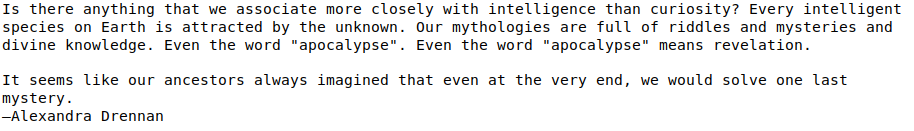
\includegraphics[width=1.0\textwidth]{curiosity_orig.png}
\end{center}
wird mit diesem Befehl verschlüsselt:
\begin{verbatim}
    \$ java keygarantie -p "Hello World" -n 1984
    examples/origin/curiosity.txt examples/enc/curiosity.txt
    encrypting 'examples/origin/curiosity.txt' with nonce 1984...
    All done, enjoy!
\end{verbatim}
Es ergibt sich die folgende Ausgabe, die nur annähernd dargestellt werden kann:
\begin{center}
    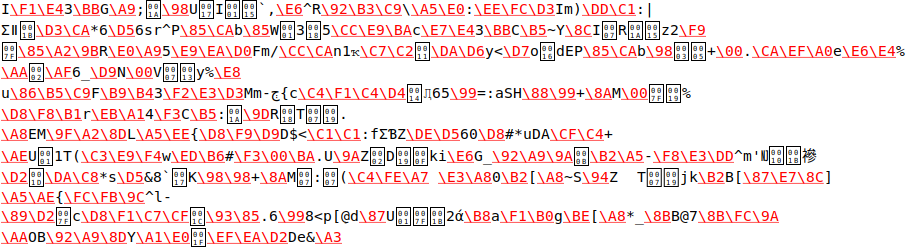
\includegraphics[width=1.0\textwidth]{curiosity_enc.png}
\end{center}
Nun wird mit dem folgenden Befehl die Datei wieder entschlüsselt:
\begin{verbatim}
    \$ java keygarantie -p "Hello World" -n 1984
    examples/enc/curiosity.txt examples/dec/curiosity.txt
    encrypting 'examples/enc/curiosity.txt' with nonce 1984...
    All done, enjoy!
\end{verbatim}
Der originale Text ist so nun wieder lesbar:
\begin{center}
    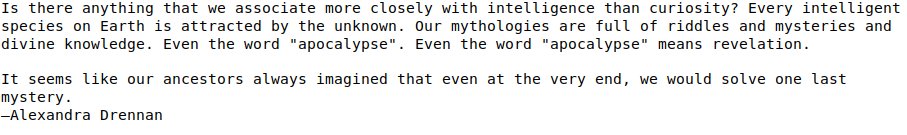
\includegraphics[width=1.0\textwidth]{curiosity_dec.png}
\end{center}

\subsection{Videodatei}

Die oben genannten Befehle werden mit angepassten Dateipfaden auf die Videodatei \textit{cute\_cat.mp4}, die sich in dem Unterordner \textit{examples/orig} befindet.
Wie erwartet, ist die verschlüsselte Datei nicht lesbar, die entschlüsselte hingegen ist es.
Diese finden sich in den Unterordnern \textit{examples/enc} respektive \textit{examples/dec}.

\section{Fazit}

\paragraph{Vorteile}
\begin{itemize}
    \item Das gleiche Verfahren kann zur Ver- und Entschlüsselung verwendet werden.
    \item Keygarantie kann mit jeglichen Dateiformaten umgehen.
    \item Selbst bei teilweiser Kompromittierung des Schlüsselstroms können keine weiteren Bereiche durch einen Angriff entschlüsselt werden.
          Replay Angriffe sind praktisch unmöglich.
    \item Es können Streams ver- und entschlüsselt werden.
    \item Der Nutzer kann zu einem beliebigen Teil des Streams springen.
    \item Der lineare Kongruenzgenerator stellt eine Erweiterung zu ChaCha dar und garantiert weitere Sicherheit.
    \item Viele Parameter, wie die Blockgröße, die Passphrasenlänge oder die mathematischen Konstanten im linearen Kongruenzgenerator, sind ohne großen Aufwand leicht veränderbar.
    \item Die Laufzeit wächst linear mit der Länge des Klartextes.
    \item Es können jegliche mit ASCII repräsentierbare Zeichen für die Passphrase verwendet werden.
\end{itemize}

\paragraph{Nachteile}
\begin{itemize}
    \item Keygarantie verwendet im Vergleich mit ChaCha 16-bit statt 32-bit Wörter in der Matrix.
    \item Die verwendete Implementation verwendet unter Umständen für mehrere Dateien die gleiche Nonce.
\end{itemize}

Keygarantie ist ein experimentelles, nicht empfohlenes Verschlüsselungsverfahren, das viele Aspekte von ChaCha übernimmt, abwandelt und erweitert.
Für die praktische Verwendung im Secure Socket Layer ist es ausdrücklich nicht empfohlen, da weitreichende Kryptoanalysen noch nicht durchgeführt wurden.

Ausschließlich für die in RFC 1149 standardisierte Übertragung von IP Datagrams\cite{Waitzman1990} ist dieses Verfahren vertretbar und empfohlen.

\bibliography{database}{}
\bibliographystyle{alpha}

\end{document}
